\chapter{Relativité restreinte}

\section{Définition relativiste de la longueur}
%%%%%%%%%%%%%%%%%%%%%%%%%%%%%%%%%

Considérons une tige AB et un tube CD.

\begin{center}

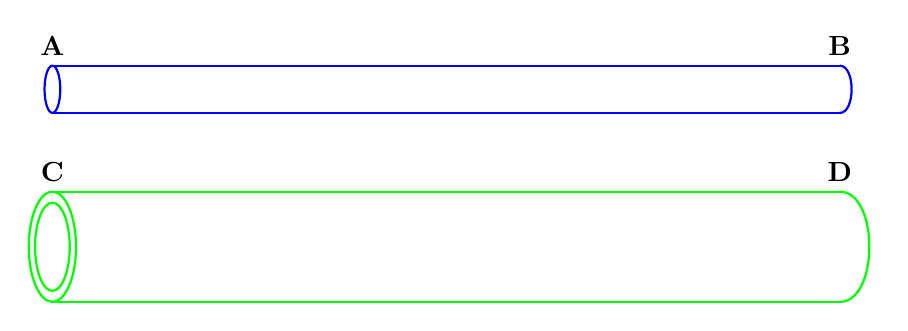
\begin{tikzpicture}
\draw (0,0.3) node [above] {{\bf A}};
\draw (10,0.3) node [above] {{\bf B}};
\draw[thick, blue] (0,0) ellipse (0.1cm and 0.3cm);
\draw[thick, blue] (0,0.3) -- (10,0.3);
\draw[thick, blue] (0,-0.3) -- (10,-0.3);
\draw[thick, blue] (10,0.3) .. controls (10.2,0.3) and (10.2,-0.3) .. (10,-0.3);

  \begin{scope}[xshift=0 cm,yshift=-2 cm]%, scale = 0.3
\draw (0,0.7) node [above] {{\bf C}};
\draw (10,0.7) node [above] {{\bf D}};
\draw[thick, green] (0,0) ellipse (0.3cm and 0.7cm);
\draw[thick, green] (0,0) ellipse (0.22cm and 0.56cm);
\draw[thick, green] (0,0.7) -- (10,0.7);
\draw[thick, green] (0,-0.7) -- (10,-0.7);
\draw[thick, green] (10,0.7) .. controls (10.5,0.7) and (10.5,-0.7) .. (10,-0.7);
  \end{scope}
\end{tikzpicture}
\end{center}

Supposons que lorsque la tige se rouve dans le tube, les extrémités de ces deux "solides" se correspondent. On peut alors dire que la tige et le tube sont de même longueur.

\begin{center}
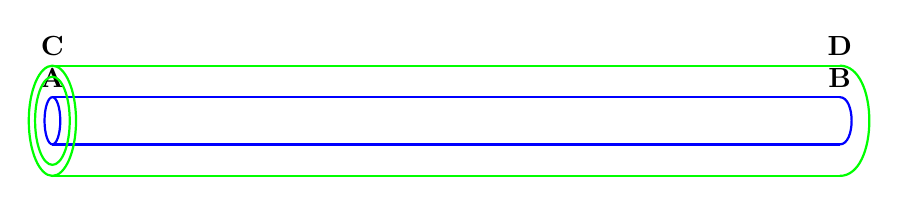
\begin{tikzpicture}
\draw (0,0.3) node [above] {{\bf A}};
\draw (10,0.3) node [above] {{\bf B}};
\draw[thick, blue] (0,0) ellipse (0.1cm and 0.3cm);
\draw[thick, blue] (0,0.3) -- (10,0.3);
\draw[thick, blue] (0,-0.3) -- (10,-0.3);
\draw[thick, blue] (10,0.3) .. controls (10.2,0.3) and (10.2,-0.3) .. (10,-0.3);
\draw (0,0.7) node [above] {{\bf C}};
\draw (10,0.7) node [above] {{\bf D}};
\draw[thick, green] (0,0) ellipse (0.3cm and 0.7cm);
\draw[thick, green] (0,0) ellipse (0.22cm and 0.56cm);
\draw[thick, green] (0,0.7) -- (10,0.7);
\draw[thick, green] (0,-0.7) -- (10,-0.7);
\draw[thick, green] (10,0.7) .. controls (10.5,0.7) and (10.5,-0.7) .. (10,-0.7);
\end{tikzpicture}
\end{center}

%Une régle graduée permet de mesurer la longueur de la tige : A étant placé en face de la graduation 0, la graduation en face de B nous donne la longueur.

Le problème c'est que lorsque l'on observe A et C au même endroit à un certain moment, rien ne nous dit que B et D sont au même endroit à ce même moment. Et si l'on va voir B et D et que l'on constate qu'il sont au même endroit à ce moment là, rien ne nous dit que A et C sont toujours au même endroit.

D'où la définition : la tige et le tube sont de même longueur si A est en face de C et B est en face de D au {\bf même moment}, en {\bf même temps}.

En physique relativiste, les évenements sont des points de l'espace-temps à 4 dimensions.
On peut alors définir l'évenement E$_1$ : A est en face de C, et l'évenement E$_2$ : B est en face de D, et la définition devient : la tige et le tube sont de même longueur si E$_1$ et E$_2$ sont {\bf simultané} (ils ont lieu au même moment). Afin de vérifier cette simultanéité, on doit placer à chaque extrémités du tube, un observateur munit d'une horloge.

\section{Relativité de la simultanéité}

A présent la tige est en mouvement. Elle se déplace à la vitesse {\bf V}. Les deux observateurs sont en place (en C et en D) et relèvent le moment, l'instant (l'heure de leur horloge) des évènements E$_1$ et E$_2$. On compare les résultats observés et on constate que E$_1$ a lieu avant E$_2$ ! Autrement dit, il semble que la tige est plus courte que le tube. Ce phénomène est généralement nommé "contraction des longueurs" mais il vaut mieux l'appeler "relativité de la simultanéité" : 
\begin{center}
\fbox{%
\begin{minipage}{0.75\textwidth}
Deux évenements, espacé par une certaine distance, étant simultané dans un certain référentiel ${\mc R}$, ne sont pas simultanés dans un référentiel ${\mc R'}$ en mouvement par rapport à ${\mc R}$
\end{minipage}
}
\end{center}

Le formalisme de la relativité permet d'obtenir une expression de la contraction des longueurs : 
\[
l'=l\sqrt{1-v^2/c^2}
\]

\begin{center}
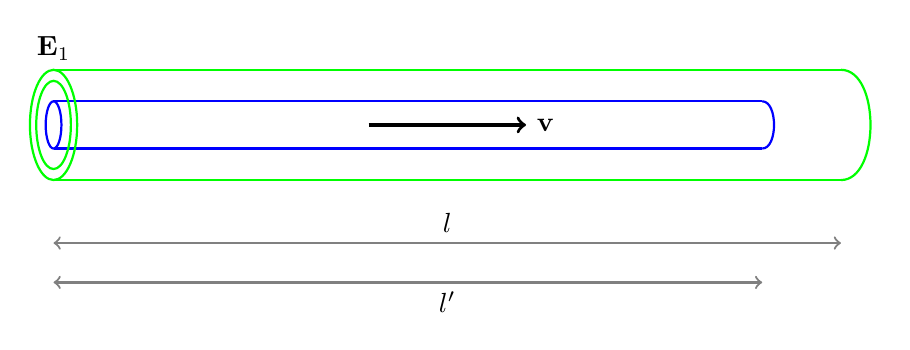
\begin{tikzpicture}
\draw[thick, blue] (0,0) ellipse (0.1cm and 0.3cm);
\draw[thick, blue] (0,0.3) -- (9,0.3);
\draw[very thick, ->] (4,0) -- (6,0) node [right] {\bf{v}};
\draw[thick, blue] (0,-0.3) -- (9,-0.3);
\draw[thick, blue] (9,0.3) .. controls (9.2,0.3) and (9.2,-0.3) .. (9,-0.3);
\draw (0,0.7) node [above] {{\bf E$_1$}};
\draw[thick, green] (0,0) ellipse (0.3cm and 0.7cm);
\draw[thick, green] (0,0) ellipse (0.22cm and 0.56cm);
\draw[thick, green] (0,0.7) -- (10,0.7);
\draw[thick, green] (0,-0.7) -- (10,-0.7);
\draw[thick, green] (10,0.7) .. controls (10.5,0.7) and (10.5,-0.7) .. (10,-0.7);
\draw[thick, <->, gray] (0,-1.5) -- (10,-1.5);
\draw (5,-1) node [below] {$l$};
\draw[thick, <->, gray] (0,-2) -- (9,-2);
\draw (5,-2) node [below] {$l'$};
\end{tikzpicture}
\end{center}


\begin{center}
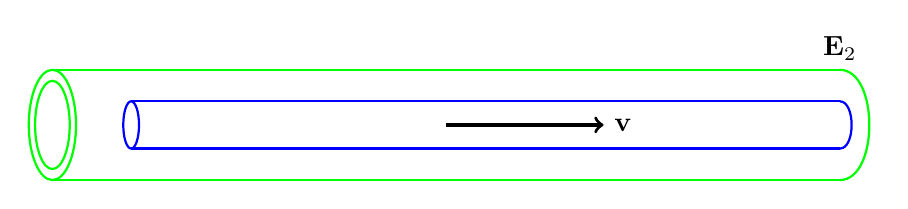
\begin{tikzpicture}
\draw[thick, blue] (1,0) ellipse (0.1cm and 0.3cm);
\draw[thick, blue] (1,0.3) -- (10,0.3);
\draw[thick, blue] (1,-0.3) -- (10,-0.3);
\draw[very thick, ->] (5,0) -- (7,0) node [right] {\bf{v}};
\draw[thick, blue] (10,0.3) .. controls (10.2,0.3) and (10.2,-0.3) .. (10,-0.3);
\draw (10,0.7) node [above] {{\bf E$_2$}};
\draw[thick, green] (0,0) ellipse (0.3cm and 0.7cm);
\draw[thick, green] (0,0) ellipse (0.22cm and 0.56cm);
\draw[thick, green] (0,0.7) -- (10,0.7);
\draw[thick, green] (0,-0.7) -- (10,-0.7);
\draw[thick, green] (10,0.7) .. controls (10.5,0.7) and (10.5,-0.7) .. (10,-0.7);
\end{tikzpicture}
\end{center}


\subsection{Chevauchons le photon}
Que se passerait-il si nous nous déplacions à la vitesse de la lumière ? que verrions nous ? Nous allons explorer cette question à partir de la formule exprimant la contraction des longueurs.


\subsection{}
\section{Conclusion}
Dans le rédérentiel du vaisseau, on mesure la vitesse de la lumière du rayon provenant du soleil et on trouve c.
Autrement dit, nous sommes Achile et nous voyons la tortue gagner la course. On a beau courir après la lumière, celle-ci a toujours cette vitesse c par rapport à nous. On a beau accélérer, augmenter notre vitesse, la lumière a toujours cette vitesse c par rapport à nous

\begin{itemize}[leftmargin=1cm, label=\ding{32}, itemsep=1pt]
\item {\bf :}
\end{itemize}

